\documentclass[UTF8,a4paper]{ctexart}

\usepackage[margin=1in]{geometry}
\usepackage{pythonhighlight}
\usepackage{amsmath}
\usepackage{float}
\usepackage{tikz}
\usepackage{url}
%\usepackage{minted}
\usetikzlibrary{shapes.geometric, arrows}
\usepackage{listings}
\lstset{basicstyle=\ttfamily,
  showstringspaces=false,
  commentstyle=\color{red},
  keywordstyle=\color{blue}
}

% 流程图定义基本形状
\tikzstyle{startstop} = [rectangle, rounded corners, minimum width=3cm, minimum height=1cm,text centered, draw=black, fill=red!30]
\tikzstyle{io} = [trapezium, trapezium left angle=70, trapezium right angle=110, minimum width=3cm, minimum height=1cm, text centered, draw=black, fill=blue!30]
\tikzstyle{process} = [rectangle, minimum width=3cm, minimum height=1cm, text centered, draw=black, fill=orange!30]
\tikzstyle{decision} = [diamond, minimum width=3cm, minimum height=1cm, text width=2cm, text centered, draw=black, fill=green!30]
\tikzstyle{arrow} = [thick,->,>=stealth]

\title{英文单词拼写错误自动检查系统 \\
\Large 自然语言处理课程设计}
\author{包利强 201628008629002 \\
雷雪林 2016E8007361072 \\
戴君义 2016E8008661015}
\date{\today}

\begin{document}
\maketitle
\tableofcontents

\clearpage
\section{课题简介}
\label{intro}
在英语写作中,单词的拼写错误是一种较为常见的错误,因此英文单词自动纠错的研究成为了自然语言处理技术的重要子课题。课题11要求我们实现一个英文文本中单词拼写错误自动检查系统,如果在检查的同时还要求进行纠错错,那么这个系统将包括两个基本的部分,即检错(detecting)和纠错(correcting)。在现代自然语言处理的研究中,英文单词拼写纠错系统又可以按照不同的情境分别进行研究,其一是\textit{上下文无关单词的检错和改错(context-free word error detection and correction or isolated-word error detection and correction)},在该情境下,每个单词的检查都是与它的上下文环境相独立的,为了检测该单词是否正确,很自然的一个做法是在词典中搜索该单词,如果搜索成功则拼写正确,否则错误,在这种方法中,算法对词典非常敏感。然而这个方法的一个很大的缺点是无法对那些拼写正确但是不符合上下文的单词进行检错,因此\textit{依赖上下文的检错和改错(context-dependent error detection and correction)}也是一个非常重要的研究课题,但由于这个课题需要语法相关的分析,因此比较复杂\cite{deorowicz2005correcting}。

\section{项目目标}
\label{target}
目前在自然语言处理研究中,拼写检查和纠错方面的研究已经进行了很长一段时间,有了很多成果和基础,也有了不少开源的拼写检查与纠错的成熟系统,主要以GNU Aspell和Hunspell为代表。我们小组在阅读相关文献和实践的基础上,将动手实现一个简单的类GNU Aspell\cite{atkinson2011gnu}系统,由于在\ref{intro}中所解释的原因,我们将只实现上个一下文无关的单词检错和改错系统。拼写错误改错意味着要对文本中出现的错误单词提供可能的正确单词建议,一般是一个概率递减的建议列表,但在自动改错时,我们只选择概率最大的一个单词替换错拼单词即可。为了方便表述,我们将这个简单的拼写纠错器称为Bspell。

\section{国内外相关工作}
\label{related}

\subsubsection{拼写纠错相关数据结构}
\label{detection}
如\ref{intro}中所说,检测一个单词是否拼写错误看起来非常简单,我们只需要在一个词典中对该单词进行查询即可,但这个方法同时也有很大的问题,首先\textit{一个包含所有正确单词的词典文件可能会非常大},查询会造成非常糟糕的空间和时间复杂度;其次,\textit{错误的拼写在很多时候会产生可以在词典中查询到的正确单词},这种情况叫做\textbf{真词错误};最后,\textit{过大的词典文件会包含很多怪异的单词},这会增加产生真词错误的可能。

20世纪80年代末到90年代初,有研究者发现,对于不同的语言,所需要的适当的词典大小是不同的,对于屈折度不高的语言如英语来说,包含50000-200000单词的词典的效果是较好的\cite{damerau1989examination,damerau1990evaluating,peterson1986note}。而对于其他一些屈折度较高的语言,所需要词典的大小可能会非常大。

在经典的数据结构中,可以满足词典的快速查询的一个实现是哈希表\cite{knuthart}。但传统的哈希表具有的一个缺点是哈希函数的选择和合适的表规模设置,否则会产生严重的碰撞问题。1997年,Czech等人\cite{czech1997perfect}所提出的最小完美哈希(minimal perfect hashing)解决了碰撞的问题,但同时也要求一个非常大的基本上和词典规模相当的哈希表。

另外一个经常用来存储词典的数据结构是前缀树(Trie)\cite{knuthart}。这是一种有序树,用于保存关联数组,其中的键通常是字符串,与二叉查找树不同,键不是直接保存在节点中,而是由节点在树中的位置决定。前缀树能够有效加速词典的查询,但它的大小也是依赖于词典的大小,为了减小前缀树的规模,很多研究者也做出了自己的努力,如著名的C-trie\cite{maly1976compressed},PATRICIA\cite{morrison1968patricia},以及Bonsai\cite{darragh1993bonsai}。

也有研究者使用一种无环确定性有限自动机(Acyclic Deterministic Finite Automaton,ADFA)\cite{deorowicz2005correcting},可以看做是前缀树的扩展。如果一颗完全前缀树的等价子树已经全部合并,那么我们就得到了一颗极小ADFA,其基本思想与前缀树类似。

还有一种方法是直接保存每个单词的词根和相应的生成规则,这样我们就知道了怎么生成每个单词的正确形式。这种方法广泛使用在开源的拼写检查器如Ispell\cite{gorin19712003}和Aspell\cite{atkinson2011gnu}中。如在Ispell中的一些例子:boolean/S,这意味着这个单词的复数形式booleans也是正确的;frizzle/DGS,则意味着frizzle,frizzled,frizzles,以及frizzling都是正确的。

\subsubsection{独立单词拼写纠错}
独立单词的纠错意味着要为\textbf{非词错误}提供一个或多个正确的单词建议,如果有多个建议,则它们应该按照可能性大小依次排序。如对于一个非词错误\textit{speling},\textit{spelling}比\textit{spilling}可能性更大,但是也不能完全确定。

一种最简单的方法是基于这样一个假设:人们在打字时通常只会犯几种错误,因此对每一个错误单词,我们需要弄明白使用一个正确单词来产生它的最小的基本操作数(如插入、删除和替换),所需的步数越小,则该正确单词产生它的概率越大。这个方法叫做最小编辑距离(minimal edit distance)方法\cite{damerau1964technique},Damerau提出后又由Wagner作了进一步研究\cite{wagner1974string}。1966年,一种建立在插入、删除和移位操作上的相似方法被提出\cite{levenshtein1966binary}。但是这种方法只能解决三大拼写错误中的一种,即\textbf{误敲},而不能同时解决其他错误。一种直接的实现方法是对词典中的每一个单词都和非词错误进行对比,这种作法比较耗时;一种更快的做法\cite{baeza1998fast}可以使得词典中要进行比较的单词数量减少一个数量级,如果非词中的错误个数较小的话。

在\textbf{相似性键技术(similarity key technique)}中,词典中的每个单词都被赋予一个键,在和非词的比较中,只有键才会进行比较,那些和非词的线索非常相似的键对应的单词会被选为建议单词。由于只有相似的键才会参与比较,所以这个方法更加有效。这个方法首先是基于SOUNDEX系统\cite{odell1918soundex}提出的,这个系统是用来对按发音转译的名字进行纠错。后来,一个相似的但是更加准确的方法被开发出来,称为SPEEDCOP\cite{pollock1984system}。这个系统提供了两种线索的实现,即概要(skeleton)和省略(omission)。但这种方法只适应于误敲的情况。

基于规则(Rule-based)的方法适用于更加普遍的错误类型,这种方法考虑的是非词向词典中正确单词的转变。第一个基于知识的系统提出于1983年\cite{yannakoudakis1983intelligent,yannakoudakis1983rules},所依赖的规则是从1000个拼写错误中得到的。这种方法有两个问题,首先是\textit{知识或规则必须通过对真实拼写错误进行实验才能得到,并且必须融合进算法之中},其次是\textit{对所获得的单词列表进行验证,判断它们是否属于词典非常困难},这使得整个过程非常耗时。但是这种方法具有的一个很好的优点是它对所有三种拼写错误都能进行处理。

在基于概率的方法(Probabilistic techniques)中,不同的编辑操作产生错误的概率是不同的。对字母替代、字母插入、字母删除和字母移位这些基本操作的的概率研究构成的概率方法的基础。在Church和Gale提出的算法\cite{church1991probability}中,这些单词通过分析语料库中的大量的单词获得,建议单词是按照生成非词的概率大小来进行排序的。

语音相似性(phonetic similarity)方法适用于对拼写错误的单词进行纠错。这种方法有一个假设,即是打字者确切地知道所要打的单词的发音,但是不知道正确的拼写方式,这样的人常常使用不正确的字形来表达音素。语音相似性可以有很多种表达方式,如SOUNDEX编码\cite{odell1918soundex}即是一种,其他的如PHONIX\cite{gadd1990phonix},MetaPhone\cite{philips1990hanging},以及Double MetaPhone\cite{philips2000double}。

\section{系统主要模块流程}

通过对相关文章的调研,我们组提出的自动纠错系统主要分为两个模块,即\textbf{检错系统}和\textbf{纠错系统}。检错系统所使用的算法为\textbf{哈希表匹配法},而纠错所使用的算法主要是\textbf{基于最长公共子串的Needleman-Wunsch算法}。主要的纠错流程为:

\begin{center}
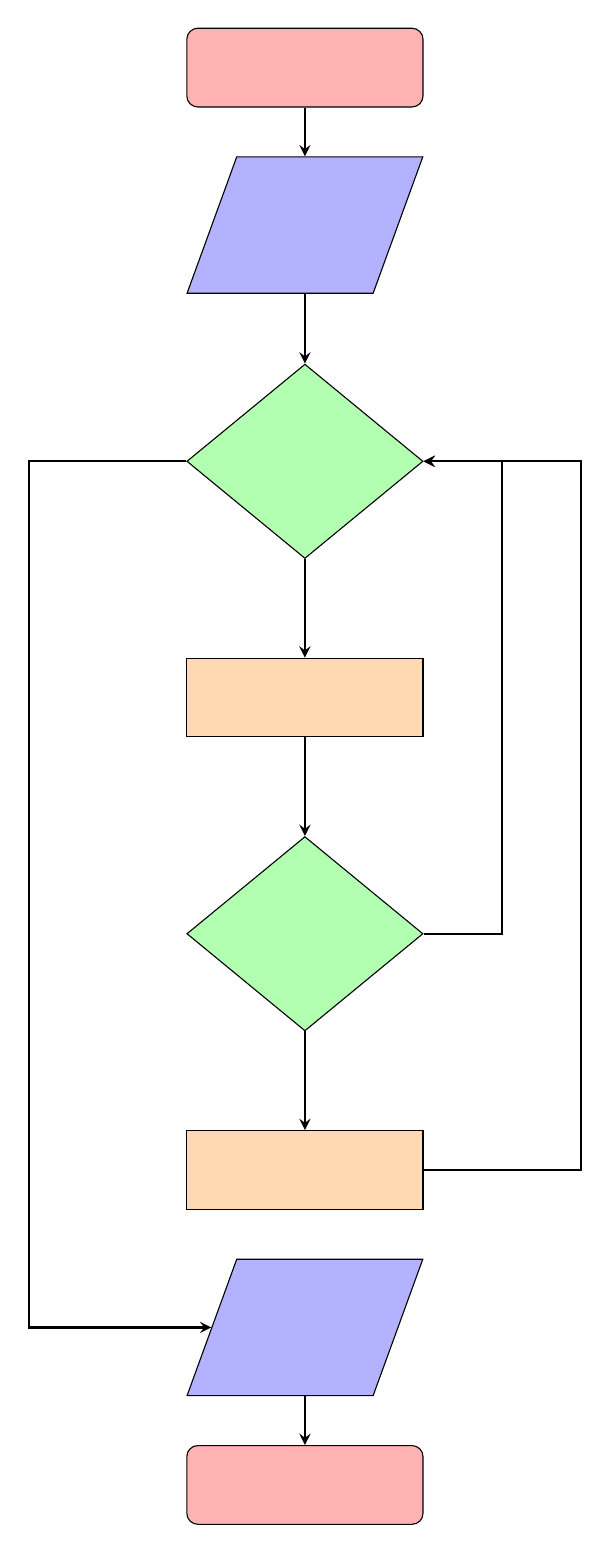
\begin{tikzpicture}[node distance=2cm]
    %定义流程图具体形状
    \node (start) [startstop] {开始};
    \node (i_text) [io, below of=start] {输入文本};
    \node (d_ok) [decision, below of=i_text, yshift=-1cm] {所有单词是否已处理?};
    \node (p_get) [process, below of=d_ok, yshift=-1cm] {获取一个单词};
    \node (d_detect) [decision, below of=p_get, yshift=-1cm] {\textbf{检错系统}是否正确?};
    \node (p_correct) [process, below of=d_detect, yshift=-1cm] {\textbf{纠错系统}};
    \node (o_writeback) [io, below of=p_correct] {写回文件};
    \node (stop) [startstop, below of=o_writeback] {停止};
     
    %连接具体形状
    \draw [arrow](start)    --  (i_text);
    \draw [arrow](i_text)   --  (d_ok);
    \draw [arrow](d_ok.west) -- ++(-2,0) node[anchor=south, pos=0.5]{是} |- (o_writeback.west);
    \draw [arrow](d_ok)     --  node[anchor=west, pos=0.5]{否} (p_get);
    \draw [arrow](p_get)    --  (d_detect);
    \draw [arrow](d_detect) --  node[anchor=west, pos=0.5]{是} (p_correct);
    \draw [arrow](d_detect.east) --  ++(1,0) node[anchor=south, pos=0.5]{否} |- (d_ok.east);
    \draw [arrow](p_correct.east) -- ++(2,0) node[anchor=south, pos=0.5]{} |- (d_ok.east);
    \draw [arrow](o_writeback) -- (stop);
\end{tikzpicture}
\end{center}

\section{核心思想和算法描述}

\subsection{检错系统}
由\ref{detection}的描述我们知道,进行单词检错最简单的一种方法是\textbf{哈希表查询法},为了实现这种技术,我们需要建立一个规模与词典大小相当的哈希表词典对象,然后将等检测的单词进行哈希匹配,如果匹配成功,则意味着待检测的单词在词形上没有错误,否则该单词拼写错误。在具体的实现过程中,我们首先使用了一个大小为69903的英文单词表,这个单词表已经足以包含我们在日常生活中所遇到的单词,但是在那些专有名词出现较多的文章中,我们建议使用专用的单词表进行代替;其次,我们使用python内置的dict数据结构来构造哈希表,因为dict的内部实现就是基于哈希函数的,这样可以在最大程度上简化我们的工作,同时还可以收到良好的效果,但有一点儿什得注意,python中的哈希函数并非前面提到的最小完美哈希函数,但对于一个具有6万多大小的列表来说,这个碰撞度是完全可以忽略的。

主要的代码如下:

\begin{python}
    def init_dict(self, voc_file):
        """
        initialize class owned dict with vocabulary file
        :param voc_file: vocabulary file
        :return:
        """
        f = open(voc_file, 'r')
        for line in f:
            tmp_line = line.strip()
            if not self.dict[tmp_line]:
                self.dict[tmp_line] = True

    def search(self, word):
        """
        search the word in the dict
        :param word: word to search
        :return: whether the word is in the dict
        """
        is_word = self.dict[word.strip()]
        if not is_word:
            self.dict.pop(word)
        return is_word
\end{python}

\subsection{纠错系统}

我们在调研的过程中发现,基于\textbf{最小编辑距离}的算法在独立单词纠错的应用中得到了广泛的应用,如非常经典的\textbf{LG算法},但与此相似的\textbf{基于最长公共子串}的算法却鲜见踪迹,因此我们决定使用基于最长公共子串的\textbf{Needleman-Wunsch算法}来完成对单词的检错工作。具体的算法描述为:

\begin{itemize}
  \item 形式化定义。 \\
  给定两个单词S和T,S的长度为m,T的长度为n,然后定义Alignment表示产生式,即单词S变成T的过程记录。我们运用最长公共子串的概念对Alignment进行打分,分数越高,则代表两个单词的相似度越高。打分原则为:

  \[
  d(S,T)=\sum_{i=1}^{min(m,n)}\delta(S[i],T[i])
  \]

  其中,关于$\delta(S[i],T[i])$我们有三种情况:如果S的第$i$个字符与T的第$i$个字符一致,则$\delta(S[i],T[i])=1$(表示得到一分);如果不一致,则$\delta(S[i],T[i])=-1$;如果少敲(如S的第$i$个字符多了出来),则$\delta(S[i],T[i])=-3$。

  举一个简单的例子为:

  \[
  \begin{aligned}
    & S: OC-URRA-NCE \\
    & T: OCCU-PATION-
  \end{aligned}
  \]

  \[
  {\rm{Alignment:}} d(S,T)=1+1-3+1-3-3-1+1-3-3-3+1-3-3=-20
  \]

  Alignment十分重要,它不仅可以识别词典中的相似度高的单词,还可以记录两个单词之间出现错误的具体信息。

  \item 动态规划求解。 \\
  形式化定义以后,我们求两个英文单词的相似度的问题就转换成了有两个字符串S和T,我们应该如何对其进行加空格使得我们的得分最高的问题。我们将给出的字符串分成更小的字符串来解决会更加方便。首先考虑最后的一个字母,假设S单词的最后一个字母为a,这个a通过T变换有三种情况:

  \begin{enumerate}
    \item 如果T的最后一个单词也是a,则他们进行匹配了;
    \item 如果a是我们多敲的,则T中的a需要我们进行插入操作变换而来;
    \item 如果a是我们少敲的,则T中的a需要我们进行删除操作变换而来。
  \end{enumerate}

  根据这三种情况,我们得到如下对应:

  \begin{enumerate}
    \item 如果S[m]与T[n]的最后一个单词形成匹配,则我们子问题就变成了S[1,...,m-1]与T[1,...,n-1]的对齐问题;
    \item 如果S[m]与空格匹配,则我们子问题就变成了S[1,...,m-1]与T[1,...,n]的对齐问题;
    \item 如果T[m]与空格匹配,则我们子问题就变成了S[1,...,m]与T[1,...,n-1]的对齐问题。
  \end{enumerate}

  我们将问题的最优解记为${\rm{OPT}}(i,j)=S[1\cdots i] alignment T[1\cdots j]$,我们可以得到下面的最优化子结构:

  \[
  {\rm{OPT}}(i,j)=max\begin{cases}
                       & \delta(S_i,T_j)+{\rm{OPT}}(i-1,j-1), \\
                       & \delta('-',T_j)+{\rm{OPT}}(i,j-1), \\
                       & \delta(S_i,'-')+{\rm{OPT}}(i-1,j), .
                     \end{cases}
  \]
  即枚举当前单元的三种可能,在其中取最大值就可以了。

  我们可以通过具体表格来说明打分过程: \\
  ${\rm{Alignment}}: d("OCURRANCE","OCCURRENCE")$

  \[
\begin{array}{ccccccccccc}
           & ''  & O   & C   & U   & R   & R   & A   & N   & C   & E   \\
        '' & 0   & -3  & -6  & -9  & -12 & -15 & -18 & -21 & -24 & -27 \\
        O  & -3  & 1   & -2  & -5  & -8  & -11 & -14 & -17 & -20 & -23 \\
        C  & -6  & -2  & 2   & -1  & -4  & -7  & -10 & -13 & -16 & -19 \\
        C  & -9  & -5  & -1  & 1   & -2  & -5  & -8  & -11 & -14 & -17 \\
        U  & -12 & -8  & -4  & 0   & 0   & -3  & -6  & -9  & -12 & -15 \\
        R  & -15 & -11 & -7  & -3  & 1   & 1   & -2  & -5  & -8  & -11 \\
        R  & -18 & -14 & -10 & -6  & -2  & 2   & -1  & -3  & -6  & -9  \\
        E  & -21 & -17 & -13 & -9  & -5  & -1  & 1   & -1  & -4  & -7  \\
        N  & -24 & -20 & -16 & -12 & -8  & -4  & -2  & 2   & -1  & -4  \\
        C  & -27 & -23 & -19 & -15 & -11 & -7  & -5  & -1  & 3   & 0   \\
        E  & -30 & -26 & -22 & -18 & -14 & -10 & -8  & -4  & 0   & 4 \\
\end{array}
  \]

  中间的单元都是由相邻的三个单元变换而来,我们的最后得分为4。这个得分本身有三个来源(即它的上方,左方,和左上方),我们可以通过不断回溯的方法找到其对应的alignment,使得S变成T。为了得到更加准确的评分,我们可以回溯多次,然后取平均,这样可以得到一个比较常见的模式。

  Bspell系统主要的动态规划代码为:

  \begin{python}
def match(self, s, t):
    """
    match two strings and return the final score
    :param s: string 1
    :param t: string 2
    :return: score
    """
       
    self.__init__(s, t)

    m = len(s) + 1
    n = len(t) + 1

    for i in range(m):
        self.opt[i, 0] = -3 * i
    for j in range(n):
        self.opt[0, j] = -3 * j

    for i in range(1, m):
        for j in range(1, n):
            if self.s[i - 1] == self.t[j - 1]:
                d = 1
            else:
                d = -1

            self.opt[i, j] = max(
                self.opt[i - 1, j - 1] + d,
                self.opt[i - 1, j] - 3,
                self.opt[i, j - 1] - 3)

    return self.opt[m - 1, n - 1]
  \end{python}

  用来对最长公共子串进行回溯的代码为:

  \begin{python}
def backtrack(self):
    """
    find the most possible case
    :return: the most possible case
    """
    
    i, j = len(self.s), len(self.t)
    a = b = ''

    while i != 0 or j != 0:
        if i == 0:
            j -= 1
            a += '-'
            b += self.t[j]
        elif j == 0:
            i -= 1
            a += self.s[i]
            b += '-'
        else:
            x, y, z = self.opt[i - 1, j - 1], self.opt[i - 1, j], self.opt[i, j - 1]
            if x >= y and x >= z:
                i -= 1
                j -= 1
                ts = self.s[i]
                tt = self.t[j]
                if ts == tt:
                    a += ts
                    b += tt
                else:
                    a += '*'
                    b += '*'
            elif y > z:
                i -= 1
                a += self.s[i]
                b += '-'
            elif y < z:
                j -= 1
                a += '-'
                b += self.t[j]
            else:
                if i >= j:
                    i -= 1
                    a += self.s[i]
                    b += '-'
                else:
                    j -= 1
                    a += '-'
                    b += self.s[j]

    return a[::-1], b[::-1]
  \end{python}

\end{itemize}

\subsection{一些细节}
\label{details}
\begin{itemize}
\item 建议序列二次排序。\\
经过Needleman-Wunsch算法对词典中的与错拼单词长度接近的单词进行动态规划匹配后,会产生一个排序列表,这个列表中的前几名可能与错拼单词都拥有相同长度的最长公共子串,如果直接将这个列表进行返回,效果会比较差,比如有的单词错拼字母位置靠前,而有的靠后,而人类打字的时候一般对单词的前面部分比较确定。我们对这个列表中具有相同分数的子列表进行二次排序,使得错拼位置靠后的单词排序靠前,这样会比较符合实际情况。

\begin{python}
# sort by score
result_list = sorted(result_dict.items(), key=lambda x: x[1], reverse=True)
result_list = result_list[:50]

# Sort again
optimal = []
len_opt = 0
for i in range(len(result_list)):
    if result_list[i][1] != result_list[0][1]:
        break
    optimal.append([result_list[i][0], 0])
    len_opt += 1

# sort the optimal by likelihood
for i in range(len(optimal)):
    optimal[i][1] = self.cmp(word, optimal[i][0])
optimal.sort(key=lambda x: x[1], reverse=True)

# the final list
final = [x[0] for x in optimal]
resdue = [x[0] for x in result_list[len_opt:]]
final.extend(resdue)
\end{python}

\item 部分词典比对。\\
词典中的单词数量一般非常多,如果直接将每一个单词都拿来与错拼单词进行最长公共子串的求解,则非常耗时,而且也没有必要,因为我们在打字的过程中很难将一个单词错打为一个比它短得多的序列,或者是比它长得多的单词,因此这个技巧是有一定道理的。在这里我们使用了一个非常简单的加速技巧,就是只将长度和错拼单词相差为$N$的单词作匹配,在代码的具体实现中,我们取$N=2$。

\begin{python}
nw = NWMatcher()
result_dict = {}

for item in self.dict:
    if not m - 2 < len(item) < m + 2:
        continue
    result_dict[item] = nw.match(word, item)
\end{python}

\end{itemize}

\section{代码运行简述}

\begin{itemize}
    \item 使用概述: \\
    我们的自动纠错系统Bspell使用python3代码写成,当安装完成相应的依赖包后就可以进行测试。代码运行时,获取指定的输入文件,该输入文件应该是包含单词拼写错误的英文文本,而且字符编码必须是\textit{UTF-8}格式。首先我们会将文本中的所有单词进行检测并保存到一一个列表中,通过检错和纠错算法循环地对每一个单词进行处理,完成所有单词的处理之后,将每个错误单词对应的建议单词写入到原文本中相应错误单词的后面(用括号分隔表示,同时在错误单词前面用\#号标记)。由于python是解释性语言,整个过程对于较大的文本可能会有一点儿延时。
  \item 环境要求: \\
  \textbf{python3}编程环境,包含\textbf{optparser}和\textbf{numpy}包。
  \item 运行方法: \\
  进入主目录,运行 \\
  \quad \textbf{python main.py} \\
  仅仅通过上述方法调用将默认纠错建议词数为1,同时将使用主目录下的\textit{input.txt}文件作为输入,而纠错的结果将自动输出到\textit{output.txt}文件中。为了可以自由地定义输入和输出文件,并指定纠错建议的个数,可以通过除加命令行参数的方法进行调用,参数介绍为: \\
  \quad \textbf{python main.py -help}

  \begin{tabular}{|l|l|l|l|}
    \hline
    % after \\: \hline or \cline{col1-col2} \cline{col3-col4} ...
    缩写 & 全写 & 默认 & 简介 \\
    -i & --input & input.txt & 指定输入文件 \\
    -o & --output & output.txt & 指定输出文件 \\
    -n & --num\_advice & 1 & 建议词的数量  \\
    \hline
  \end{tabular}

  完全的调用方式为: \\
  \quad \textbf{python main.py -i in\_file -o out\_file -n 2}
\end{itemize}

\section{系统评测}

GNU Aspell\cite{atkinson2011gnu}是一个免费开源的拼写检查器,它的设计初衷是为了取代已经过时的Ispell\cite{gorin19712003},和我们所设计的简单的Bspell系统一样,它的功能也是为英文文本提供拼写检查和可能的正确单词建议。GNU Aspell的设计者为这个系统设计了一个非常合理的性能检测方法,并与之前所出现的一些主要的拼写检查器进行了比较,在此,我们将沿用这个方法,并使用同样的测试数据,以便对我们所完成的系统进行真实合理的评测,并在和主流系统的对比中了解我们设计的框架的合理性。

\subsection{测试数据}

Aspell所用的测试数据包含546个错误拼写的单词以及它们相应的正确形式,每个错拼单词和正确单词在文件中占一行,因此文件一共包括546行,文件所在的网址为\url{http://aspell.net/test/cur/batch0.tab}。在测试的过程中,为了排除字典文件带来的性能误差,和Aspell一样,我们只对其正确形式在词典中可以找到的单词进行统计,这样所涉及的误拼单词的规模对Bspell来说是478,而对Aspell来说是493,我们假设这个很小的不同对评测结果没有本质上的影响。

\subsection{评测标准}

Aspell的评测项共有8个,分别是:

\begin{itemize}
\item Total (T)。Total是指测试集中误拼单词的正确形式在字典中能够查到的误拼单词集合或其大小,因为只有正确形式出现在字典中的单词,我们才有可能进行正确的预测;
\item Rank1 (R1)。第一个建议预测正确的个数;
\item Rank5 (R5)。前5个建议中预测正确的个数,以下Rank10,Rank25,Rank50类似;
\item Total Found (TF)。Total中的误拼单词被正确预测的个数(Rank1-Rank50可以找到);
\item Total Not Found (TNF)。没有预测正确的单词个数;
\item Score。定义为$\frac{Total Found}{Total} \times 100\%$。
\item Time。评测过程进行的时间。
\end{itemize}

\subsection{评测结果}

我们按照上述写了一个简单的评测代码,对BSpell系统进行了评测,代码命名为\textit{test.py},包含在项目目录中。评测得到的结果为:

\begin{table}[hbp]
\centering
    \begin{tabular}{|l|l|l|l|l|l|l|l|l|l|}
    \hline
		~ & Score & TNF & TF & R1 & R5 & R10 & R25 & R50 & Time (min) \\
		\hline
		Aspell .31 / Normal & 93.1 &34 & 459 &59.6 & 85.6 & 90.1 & 92.9 & 93.1 & 3.58 \\
		\hline
		Aspell .33 / Normal		&91.7	&41			&452		&57.0	&80.9	&88.0	&91.1	&91.5 & 29.46 \\
		\hline
		Aspell 0.50 / Normal		&91.9	&40			&453		&57.2	&81.1	&88.4	&91.5	&91.7 & 24.02 \\
		\hline
		Aspell 0.60 / Normal		&89.0	&54			&439		&53.1	&79.7	&86.2	&88.4	&89.0 & 0.69 \\
		\hline
		Aspell 0.60 / Slow		&93.1	&34			&459		&53.3	&80.7	&89.0	&92.5	&93.1 & 4.82 \\
		\hline
		Aspell 0.60.6 / Normal		&89.7	&51			&442		&53.3	&80.1	&86.8	&89.0	&89.7 & 1.18 \\
		\hline
		Aspell 0.60.6 / Slow		&92.9	&35			&458		&53.3	&80.5	&88.8	&92.3	&92.9 & 5.26 \\
		\hline
		Hunspell 1.1.12			&81.7	&90			&403		&55.2	&78.1	&80.7	&81.7	&81.7 & 24.39 \\
		\hline
		Hunspell w/ Phonetic Lookup	&85.6	&71			&422		&56.0	&81.9	&85.2	&85.6	&85.6 & 42.16 \\
		\hline
		Ispell 3.1.20 w/ -S option	&54.8	&223			&270		&38.3	&51.9	&54.0	&54.8	&54.8 & 0.15 \\
		\hline
		Word 97				&72.2	&137			&356		&59.0	&70.8	&72.2	&72.2	&72.2  & ~ \\
		\hline
		\textbf{Bspell}	 &	81.4 & 89 & 389 & 50.0 & 66.1 & 73.0 & 79.3 & 81.4 & 30.0 \\
		\hline
    \end{tabular}
\end{table}

根据这个评测结果,我们可以看到Bspell系统大概和Hunspell 1.1.12的性能处于相同级别,相对于最新版的Aspell拼写检查器来说还远远落于下风。当然,Aspell是一个已经非常成熟的拼写检查器,在众多的编辑器如emacs和vim中都可以看到它的身影,因此这个结果也是在意料之中的。

\section{组员分工}

\subsection{包利强}

\begin{itemize}
\item 阅读了3篇比较典型的文献以用GNU Aspell的文档;
\item 与小组成员一起讨论提出了Bspell系统的模块以及流程;
\item 完成了报告的第5、6、7部分;
\item 完成了Bspell的代码编写工作;
\end{itemize}

\subsection{雷雪林}

\begin{itemize}
\item 阅读了6篇相关的文章,并在前期进行了比较全面的调研;
\item 讨论提出了Bspell系统的模块以及流程;
\item 完成了报告的第3、4部分;
\item 提出了\ref{details}中的二次排序方法。
\end{itemize}

\subsection{戴君义}

\begin{itemize}
\item 阅读了4篇相关方面的文献;
\item 讨论提出了Bspell系统的模块以及流程;
\item 完成了报告的第1、2部分;
\item 提出了\ref{details}中的部分匹配方法。
\end{itemize}

\section{总结}

本次课程设计是应完成国科大所开设的自然语言处理课程的要求而进行的,在此,我们感谢所有的老师给予我们这次珍贵的锻炼机会。单词的自动拼写检查在自然语言处理中是一项非常基础的工作,自然语言处理的大部分工作都要求在无错误的拼写基础上进行,而同时,自然语言中的文法分析等任务的进展又反过来促进了单词自动拼写检查的发展,如N-gram在形式正确而上下文错误的拼写纠错中的应用。

从本次课程设计中来看,我们在知识储备、学习方法、思考方式以及编程能力等方面仍然有着很大的缺陷,在整个过程中有时千头万绪,难以理清,有时又灵感尽失,茫然无措;而系统设计混乱、细节考虑不周、乃至总体进展缓慢等问题层出不断,备感无力。好在高朋相伴,文海作陪,终于克期而成,虽差强人意,却也不孚所望。总之,此次课程设计在一定程度上提高了整个小组的科研能力,丰富了研一的学习生活,作为最后一门考试的课程,它也名正言顺地为整个雁栖湖的研一生活划上了句号。

\clearpage
\bibliographystyle{ieeetr}
\bibliography{proofreading}
\end{document} 